\title[概率论]{第十讲:常见的连续型分布}

\institute[东南大学数学学院]{\large \textrm{Email: xzhangseu@seu.edu.cn} \\ \quad  \\
	\large 东南大学 \quad 数学学院 \\
	\vspace{0.3cm}
	%  \trc{公共邮箱: \textrm{zy.prob@qq.com}\\
	%    \hspace{-1.7cm}  密 \qquad 码: \textrm{seu!prob}}
}
\date{}


{ \setbeamertemplate{footline}{}
	\begin{frame}
		\titlepage
	\end{frame}
}

% \begin{frame}[plain]
%   \frametitle{目录}
%   \setcounter{tocdepth}{2}
%   \tableofcontents
% \end{frame}
\addtocounter{framenumber}{-3}  % 目录页不计算页码
%\section{随机变量}
\subsection{常见的连续型分布}
\begin{frame}
	\frametitle{均匀分布}
	\begin{defi}
		任给参数 $a<b$, 函数
		\begin{eqnarray*}
			p(x)=\dfrac{1}{b-a}, \quad a<x<b
		\end{eqnarray*}
		满足密度函数的两个性质即:$p (x)\ge 0$ 且 $\int_{-\infty}^\infty p (x) dx=1$. 我们称以上式中的 $p (x)$ 为密度的连续型分布为区间 $(a,b)$ 上的均匀分布,记作 $U (a,b)$.
	\end{defi}
	\pause

	\begin{itemize}[<+-|alert@+>]
		\item 易见,均匀分布的分布函数为
		      \begin{eqnarray*}
			      F(x)=\left\{
			      \begin{array}{ll}
				      0,                & x<a       \\
				      \dfrac{x-a}{b-a}, & a\leq x<b \\
				      1.                & x\ge b
			      \end{array}
			      \right.
		      \end{eqnarray*}
		\item 如果 $X$ 服从 $U (a,b)$ 分布,则对任何 $a\le x<y\le b$ 有
		      \begin{eqnarray*}
			      P(x<X\le y)=\pause \int_x^y\dfrac{1}{b-a}dt=\pause \dfrac{y-x}{b-a}
		      \end{eqnarray*}

	\end{itemize}

\end{frame}

\begin{frame}
	\begin{figure}[htbp]
		\centering
		
\includegraphics[width=8.5cm]{GaussMoney.jpg}
	\end{figure}
\end{frame}
% \setbeamertemplate{caption}[numbered]

\begin{frame}
	\begin{columns}
		\column{4cm}
		\begin{figure}[htbp]\nonumber
			\centering
			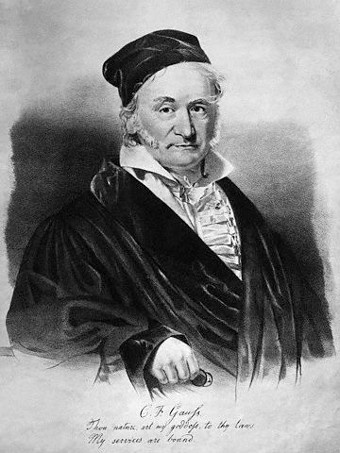
\includegraphics[width=5cm]{Gauss.jpg}
			\caption{高斯}
		\end{figure}
		\column{6cm}
		\begin{itemize}[<+-|alert@+>]
			\item 卡尔。弗里德里希。高斯 1777 年出生于布伦瑞克;
			\item 11 岁时就发现了二项式定理;
			\item 19 岁发现正十七边形的尺规作图法,解决了困扰数学家们两千多年的难题;
			\item 1809 年提出 “最小二乘法” 并在此基础上建立的正态分布方程,是概率统计中一个非常重要的工具,广泛应用于数学、物理学等领域;
			\item 一生发表了 155 篇论文,对数论、代数学、非欧几何、复变函数和微分几何等领域都做出了开创性的贡献,被誉为数学王子.
		\end{itemize}
	\end{columns}
\end{frame}
\begin{frame}
	\frametitle{正态分布 (高斯分布)}
	考虑下述函数
	\begin{eqnarray*}
		p_{\mu,\sigma}(x):=\dfrac{1}{\sqrt{2\pi}\sigma}e^{-\dfrac{(x-\mu)^2}{2\sigma^2}}
	\end{eqnarray*}
	\pause 下面我们验证 $p_{\mu,\sigma}(x)$ 满足密度函数的两个性质即非负性与正则性:非负性显然;正则性则需要计算积分 $I:=\int_{-\infty}^\infty p_{\mu,\sigma}(x) dx$.
\end{frame}

\begin{frame}
	\vspace{0.4cm}
	由于 $p_{\mu,\sigma}(x)$ 的原函数不是初等函数,我们无法通过微积分基本公式计算 $I$. 我们考虑计算 $I^2$:
	\begin{eqnarray*}
		I^2&=&\pause \int_{-\infty}^\infty \dfrac{1}{\sqrt{2\pi}\sigma}e^{-\dfrac{(x-\mu)^2}{2\sigma^2}}dx\int_{-\infty}^\infty \dfrac{1}{\sqrt{2\pi}\sigma}e^{-\dfrac{(x-\mu)^2}{2\sigma^2}}dx\\
		&=&\pause \int_{-\infty}^\infty \dfrac{1}{\sqrt{2\pi}\sigma}e^{-\dfrac{(x-\mu)^2}{2\sigma^2}}dx\int_{-\infty}^\infty \dfrac{1}{\sqrt{2\pi}\sigma}e^{-\dfrac{(y-\mu)^2}{2\sigma^2}}dy\\
		&=&\pause \int_{-\infty}^\infty\dfrac{1}{\sqrt{2\pi}}e^{-\dfrac{x^2}{2}}dx\int_{-\infty}^\infty\dfrac{1}{\sqrt{2\pi}}e^{-\dfrac{y^2}{2}}dy\\
		&=&\pause \dfrac{1}{2\pi}\int_{-\infty}^\infty\int_{-\infty}^\infty e^{-\dfrac{x^2+y^2}{2}}dxdy\\
		&=&\pause \dfrac{1}{2\pi}\int_0^{2\pi}\int_0^\infty e^{-\dfrac{r^2}{2}}rdrd\theta\\
		&=&\pause 1
	\end{eqnarray*}


\end{frame}
\begin{frame}
	\frametitle{正态分布的定义}
	\begin{defi}
		若随机变量 $X$ 的密度函数为
		\begin{eqnarray*}
			p_{\mu,\sigma}(x):=\dfrac{1}{\sqrt{2\pi}\sigma}e^{-\dfrac{(x-\mu)^2}{2\sigma^2}}
		\end{eqnarray*}
		则称 $X$ 服从参数为 $(\mu,\sigma^2)$ 的正态分布,记作 $X\sim N (\mu,\sigma^2)$. 特别的称 $N (0,1)$ 分布为标准正态分布,并简写 $p_{0,1}(x)$ 为 $\varphi (x)$. 正态分布又称高斯分布.
	\end{defi}
\end{frame}

\begin{frame}
	\frametitle{正态分布的性质}
	\begin{itemize}[<+-|alert@+>]
		\item 分布密度关于参数 $\mu$ 对称,即有
		      \begin{eqnarray*}
			      p_{\mu,\sigma}(\mu-x)=p_{\mu,\sigma}(\mu+x),  \quad \forall x \in R
		      \end{eqnarray*}
		      特别的,$N (0,1)$ 分布的密度函数为偶函数.
		\item $p_{\mu,\sigma}(x)$ 在 $x=\mu$ 处取得最大值 $\dfrac{1}{\sqrt{2\pi}\sigma}$. 注意到密度曲线下的面积应保持等于 1, 并且密度函数在 $x$ 处的值反映了此分布取值 $x$ 附近的概率大小。故 $\sigma^2$ 越小,密度的曲线越尖陡,分布取值越集中;$\sigma^2$ 越大,密度曲线越平缓,分布取值越分散.
		\item 正态分布的分布函数为
		      \begin{eqnarray*}
			      \Phi_{\mu,\sigma}(x)=\int_{-\infty}^x\dfrac{1}{\sqrt{2\pi}\sigma}e^{-\dfrac{(t-\mu)^2}{2\sigma^2}}dt
		      \end{eqnarray*}
		      特别的记标准正态分布函数为 $\Phi (x)$. 其与 $\Phi_{\mu,\sigma}(x)$ 有以下关系:
		      \begin{eqnarray*}
			      \Phi_{\mu,\sigma}(x)=\Phi(\dfrac{x-\mu}{\sigma})
		      \end{eqnarray*}
	\end{itemize}
\end{frame}
\begin{frame}
	\begin{exam}[3$\sigma$ 原则] 设随机变量 $X$ 服从 $N (\mu,\sigma^2)$ 分布,求 $P (|X-\mu|<3\sigma)$.
	\end{exam}

	\pause \jieda 注意到
	\begin{eqnarray*}
		P(|X-\mu|<3\sigma)&=&\pause P(\mu-3\sigma<X<\mu+3\sigma)\\
		&=&\pause \Phi_{\mu,\sigma}(\mu+3\sigma)-\Phi_{\mu,\sigma}(\mu-3\sigma)\\
		&=&\pause \Phi(3)-\Phi(-3)=\pause \Phi(3)-(1-\Phi(3))\\
		&=&\pause 2\Phi(3)-1=\pause 0.9973
	\end{eqnarray*}
	\pause 这表明,尽管正态分布的取值范围是 $(-\infty,+\infty)$, 但是其取值落在区间 $(\mu-3\sigma,\mu+3\sigma)$ 的概率高达 $99.73\%$


\end{frame}
\begin{frame}
	\frametitle{标准正态分布与一般正态分布之间的关系}
	\begin{exam}
		若 $X\sim N (\mu,\sigma^2)$, 则 $Y:=\dfrac{X-\mu}{\sigma}\sim N (0,1)$; 反之,若 $X\sim N (0,1)$, 则 $Y:=\sigma X+\mu\sim N (\mu,\sigma^2)$.
	\end{exam}

	\pause \jieda 我们仅给出第一种情况的证明。事实上,我们只需要说明 $Y$ 的分布密度为
	\vspace{-0.7cm}\begin{eqnarray*}
		\varphi(x)=\dfrac{1}{\sqrt{2\pi}}e^{-\dfrac{x^2}{2}}
	\end{eqnarray*}
	即可. \pause 事实上,考虑 $Y$ 的分布函数
	\begin{eqnarray*}
		F_Y(x)&=&\pause P(Y\le x)=\pause P(\dfrac{X-\mu}{\sigma}\le x)=\pause P(X\le \sigma x+\mu)\\
		&=&\pause \int_{-\infty}^{\sigma x+\mu}\dfrac{1}{\sqrt{2\pi}\sigma}e^{-\dfrac{(t-\mu)^2}{2\sigma^2}}dt=\pause \int_{-\infty}^x\dfrac{1}{\sqrt{2\pi}}e^{-\dfrac{y^2}{2}}dy
	\end{eqnarray*}
	\pause 从而 $Y$ 的分布密度为
	\begin{eqnarray*}
		p_Y(x)=F_Y'(x)=\dfrac{1}{\sqrt{2\pi}}e^{-\dfrac{x^2}{2}}=\varphi(x)
	\end{eqnarray*}
\end{frame}
\begin{frame}
	\frametitle{正态分布函数的简单性质}
	记 $\Phi (x)$ 为标准正态分布的分布函数,$U\sim N (0,1)$,  $\Phi_{\mu,\sigma}(x)$ 为 $N (\mu,\sigma^2)$ 分布的分布函数,$X\sim N (\mu,\sigma^2)$, 则 \pause
	\begin{itemize}[<+-|alert@+>]
		\item $\Phi(0)=\dfrac{1}{2}$;
		\item $\Phi_{\mu,\sigma}(\mu)=\dfrac{1}{2}$;
		\item $\Phi(-x)=1-\Phi(x)$;
		\item $P(|U|<x)=P(-x<U<x)=\pause P(U<x)-P(U\le -x)$ $=\pause \Phi(x)-(1-\Phi(x))=\pause 2\Phi(x)-1$;
		\item $\Phi_{\mu,\sigma}(x)=\pause P(X\le x)=\pause P(\dfrac{X-\mu}{\sigma}\le \dfrac{x-\mu}{\sigma})=\pause \Phi(\dfrac{x-\mu}{\sigma})$\pause
		\item $P(a<X\le b)=\Phi(\dfrac{b-\mu}{\sigma})-\Phi(\dfrac{a-\mu}{\sigma})$.
	\end{itemize}

\end{frame}
\begin{frame}
	\frametitle{伽玛函数 (Gamma 函数)}
	\begin{defi}
		称以下函数
		\begin{eqnarray*}
			\Gamma(\alpha):=\int_0^\infty x^{\alpha-1}e^{-x}dx, \quad \alpha>0,
		\end{eqnarray*}
		为 Gamma 函数.
	\end{defi}
	\pause
	Gamma 函数有以下性质:\pause
	\begin{itemize}[<+-|alert@+>]
		\item $\Gamma(1)=\pause \int_0^\infty x^{1-1}e^{-x}dx=\pause 1$;
		\item $\Gamma(\dfrac{1}{2})=\pause \int_0^\infty x^{\frac{1}{2}-1}e^{-x}dx=\pause 2\sqrt{\pi}\int_0^\infty \frac{1}{\sqrt{2\pi}}e^{-x}d\sqrt{2}x^{\frac{1}{2}}$ \pause $=2\sqrt{\pi}\int_0^\infty \frac{1}{\sqrt{2\pi}}e^{-\frac{t^2}{2}}dt=\pause \sqrt{\pi}$;
		\item $\Gamma (\alpha+1)=\alpha\Gamma (\alpha)$, 故 $\Gamma (n+1)=n\Gamma (n)=\cdots =n!$; \pause 事实上,
		      \begin{eqnarray*}
			      \Gamma(\alpha+1)&=&\pause \int_0^\infty x^\alpha e^{-x}dx=\pause \int_0^\infty -x^\alpha de^{-x}\\
			      &=&\pause -x^\alpha e^{-x}|_0^\infty+\int_0^\infty \alpha x^{\alpha-1} e^{-x}dx=\pause \alpha\Gamma(\alpha)
		      \end{eqnarray*}
	\end{itemize}

\end{frame}
\begin{frame}
	\frametitle{伽玛分布}
	\begin{defi}[Gamma 分布]
		若随机变量 $X$ 的密度函数为
		\begin{eqnarray*}
			p(x)=\left\{
			\begin{array}{ll}
				\dfrac{\lambda^\alpha}{\Gamma(\alpha)}x^{\alpha-1}e^{-\lambda x}, & x\ge 0 \\
				0,                                                                & x<0
			\end{array}
			\right.
		\end{eqnarray*}
		则称 $X$ 服从参数为 $(\alpha,\lambda)$ 的 Gamma 分布,记作 $X\sim \Gamma (\alpha,\lambda)$.
	\end{defi}
\end{frame}

\begin{frame}
	\frametitle{指数分布与 $\chi^2$(卡方) 分布}
	\begin{defi}
		称 $\Gamma (1,\lambda)$ 分布为指数分布,其密度函数与分布函数分别为
		\begin{eqnarray*}
			p(x)=\left\{
			\begin{array}{ll}
				\lambda e^{-\lambda x}, & x\ge 0, \\
				0,                      & x<0.
			\end{array}
			\right.\quad
			F(x)=\left\{
			\begin{array}{ll}
				1- e^{-\lambda x}, & x\ge 0, \\
				0,                 & x<0.
			\end{array}
			\right.
		\end{eqnarray*}

	\end{defi}
	\pause

	\begin{defi}
		称 $\Gamma (\frac{n}{2},\frac{1}{2})$ 分布为 $\chi^2$ 分布,记作 $\chi^2 (n)$, 其密度函数为
		\begin{eqnarray*}
			p(x)=\left\{
			\begin{array}{ll}
				\dfrac{1}{2^{\frac{n}{2}}\Gamma(\frac{n}{2})}x^{\frac{n}{2}-1}e^{-\frac{x}{2}}, & x\ge 0, \\
				0,                                                                              & x<0.
			\end{array}
			\right.
		\end{eqnarray*}

	\end{defi}
\end{frame}

\begin{frame}
	\frametitle{泊松分布与伽玛分布}
	\begin{exam}
		假定有一个于随机时刻陆续到来的质点流,我们若以 $N (t)$ 表示在 $[0,t]$ 时间内到来的质点的个数,并假设其服从参数为 $\lambda t$ 的泊松分布。试证明第 $n$ 个质点到达的时间 $S_n$ 服从 $\Gamma (n,\lambda)$ 分布.
	\end{exam}

	\pause
	\zheng 首先我们考虑一下 $S_n$ 的分布函数
	\begin{eqnarray*}
		P(S_n\le t)&=&\pause P(N(t)\ge n)=\pause \sum_{k=n}^\infty P(N(t)=k)\\
		&=&\sum_{k=n}^\infty \dfrac{(\lambda t)^k}{k!}e^{-\lambda t}
	\end{eqnarray*}
	\pause 故其密度 $p (t)$ 为
	\begin{eqnarray*}
		p(t)=F'(t)&=&\pause \sum_{k=n}^\infty\left[ \dfrac{\lambda(\lambda t)^{k-1}}{(k-1)!}e^{-\lambda t} - \dfrac{\lambda(\lambda t)^k}{k!}e^{-\lambda t}\right]\\
		&=& \pause \dfrac{\lambda(\lambda t)^{n-1}}{(n-1)!}e^{-\lambda t}=\pause \dfrac{\lambda^n}{\Gamma(n)}t^{n-1}e^{-\lambda t}
	\end{eqnarray*}

\end{frame}



% \input{ProbChap1.tex}

% \input{ProbChap2.tex}
% \input{ProbChap3.tex}
%  \input{ProbChap4.tex}




%%% Local Variables:
%%% mode: latex
%%% TeX-master: t
%%% End:
